


\thispagestyle{empty} 
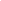
\includegraphics{Images/pixel.png}
\vfill
\parbox[b]{11cm}{\raggedright

\textcopyright {\the\year} Peter W. Brewer\\[2mm] Malcolm and Carolyn Wiener Laboratory for Aegean\\ and Near Eastern Dendrochronology \\
Cornell Tree-Ring Laboratory\\
B48 Goldwin Smith Hall\\ Cornell University \\ Ithaca, New York 14853. USA.\\[0.5cm] \Telefon\hspace{3mm}+1 607 255 8650 \\ \Letter\hspace{3mm}p.brewer@cornell.edu\\[5mm] Compiled: \today\\[10mm]}

{\footnotesize 
Permission is granted to copy, distribute and/or modify this document
under the terms of the GNU Free Documentation License, Version 1.3
or any later version published by the Free Software Foundation;
with no Invariant Sections, no Front-Cover Texts, and no Back-Cover Texts.
A copy of the license is included in the appendix entitled ``GNU Free Documentation License'' (pages \pageref{txt:FDLStart}--\pageref{txt:FDLEnd}).}



\newpage
\pagenumbering{roman}
\setcounter{page}{1}
\thispagestyle{empty} 
{ 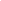
\includegraphics{Images/pixel.png}\\[4cm] 
\hrule 
\vspace{5mm}
\Huge \bfseries \thetitle\\[3mm] 
\large{\thesubtitle}
\vspace{5mm}
\hrule
\vspace{3cm}
}
{
\normalsize
\textbf{By \authornames}\\[0.6cm]
}
{
\vfill
\footnotesize
Compiled: \today
}

\newpage


\tableofcontents


\cleardoublepage
\pagenumbering{arabic} 

\phantomsection
\section*{Preface}
\thispagestyle{empty} 
\addcontentsline{toc}{section}{Preface}

Corina is the tree ring measuring and analysis program developed at the Cornell Tree-Ring Laboratory. It is focused primarily on the measurement of tree ring widths and the organization and curation of the data, metadata and physical samples. It is cross-platform (running on all Java 6 enabled operating systems including Windows, MacOSX and Linux) and open-source. It includes support for standard measuring platforms including Velmex, Lintab and Henson.

Corina has been developed since 2000 as a desktop Java application, following an earlier DOS-based version programmed in C, which itself was derived from a collection of FORTRAN and C utilities. Earlier iterations of Corina (version 0.x and 1.x) were built around a standard file-based data management system. In 2007, work began on a major rewrite of the software whereby this file-based data management was replaced with an object-relational database management system (ORDBMS) and server/client webservice infrastructure. This series of releases (versions 2.x) are what are described in this manual.  This initiative was made possible because of the support of the College of Arts \& Sciences, Cornell University, via a grant to Sturt Manning to re-envisage the Cornell Tree-Ring Laboratory, which provided support for Peter Brewer to develop Corina at Cornell University.

This manual is divided into two main sections, the first for users, the second for developers.  Corina is open source software (see the details of the license on pages \pageref{txt:licenseStart}--\pageref{txt:licenseEnd}), so you are welcome to inspect and edit the code.  The second part of this manual will help you do that.

Over the years Corina has been developed by a number of people: Peter Brewer, Chris Dunham, Aaron Hamid, Dan Girshovich, Ken Harris, Drew Kalina, Rocky Li, Lucas Madar, Daniel Murphy, Robert 'Mecki' Pohl and Kit Sturgeon.  We would like to thank the many people that have tested Corina especially: Charlotte Pearson; Carol Griggs; Brita Lorentzen; Jess Herlich; LeAnn Canady; Kate Seufer; and many undergraduate and postgradutes students at Cornell.  

We would also like to thank the College of Arts \& Sciences and the Department of Classics, Cornell University; the Malcolm H.\ Wiener Foundation; and the many patrons of the Malcolm and Carolyn Wiener Laboratory for Aegean and Near Eastern Dendrochronology for their financial support.  

We hope that you find Corina useful and look forward to hearing your feedback.  



